\chapter{Implementation}
\label{cha:implementation}

This chapter will describe in detail the technical implementation of the Omni platform.

\section{Configuration}
Configuration is an important part of any production application. It is any data required by the application for it to run.
Configuration may need to change, and it should be able to do so without requiring developers to rebuild the application.
Allowing configuration to be ephemeral enables companies with separate teams that manage a platform's operations to make configuration changes without the need for intervention by a software developer.

Configuration items should be passed to the application via its environment rather than compiled into its binary.
One method for specifying configuration is through a configuration file. This file (normally JSON or YAML) contains key-value pairs of data for the application to consume at start-up.
Some frameworks even enable the file to be monitored for changes so that the most up-to-date values can be used without requiring a restart. 

Another method preferred in Kubernetes and containerised environments is using environment variables.
These are variables set in the bash environment that the application is executed from. The application can then read the values of these variables and use them for its own configuration.

Kubernetes allows environment variables to be specified in the workload manifests for each application.
This means that if the configuration changes, a new manifest can be loaded to bring new pods online with the updated config. Once the new pods are available and responding to requests, the old pods can be scaled down and removed.

\lstinputlisting[language=Go, caption=Example of Parsing Environment Variables, label={lst:go-env}]{code-snippets/go-env-example.go}

The second method will be used as Omni is designed for Kubernetes. To enable the use of environment variables for configuration, an open-source package called \underline{\href{https://github.com/caarlos0/env}{Caarlos0/env}} \nocite{env} will automatically pull these values from the environment (shown in Listing \ref{lst:go-env}).
Defined in the applications are different configuration objects with the required configuration items included, along with some special tags that indicate the name of the related environment variable.
On start-up, a call to the package automatically creates the configuration objects based on the values from the environment. The config objects can then be passed around the application to the sections of code that require them.

\section{Observability}
Logging and observability are vital to the ongoing stability of any production system. ``The distributed nature of microservices also introduces complexity, making  it  challenging  to  ensure  the  reliability,  performance,  and  security  of  the  system'' \citep{chinamanagonda2022observability}.
Clear and consistent logs are crucial for developers to be able to debug faulty platforms quickly. 

Logging is not the only facet of observability. However, metrics and tracing are also key to building a holistic view of a platform's health.
Metrics are the key numerical data points representing a system's health and behaviour over time.
Metrics often include requests per second, latency and CPU usage. These can be easily aggregated, structured, and visualised in top-level dashboards to provide a glanceable overview of how a platform is performing.
They are the first level of reporting an operations team will monitor.

Traces, on the other hand, record the path that requests take through a platform. They often capture the logs each system produces along the way and measure latencies across the system.
Traces are ideal for identifying bottlenecks and pinpointing failures within a larger microservices architecture. Tracing is often handled by a framework called \underline{\href{https://opentelemetry.io}{Open Telemetry}} \nocite{opentel}, a standardised way of collecting and exporting traces from many different applications.

Finally, logs are the lowest level of the three fundamental observability pillars. Logs are immutable, and applications emit timestamped events to process incoming requests.
Developers with a fine-grained understanding of how the system functions best use logs, which are extremely useful for pinpointing the exact line where a system has failed. 

\subsection{Observability in Omni}
In Omni, the Go standard library's structured logger emits logs, allowing each log to contain extra information, such as variables.
The structured logger can output logs in various formats, the most common being text-based (for console logs) and JSON-based (for consumption into an observability pipeline).

\lstinputlisting[language=Go, caption=Example of Structured Logging]{code-snippets/go-logger-example.go}

\begin{figure}[htbp]
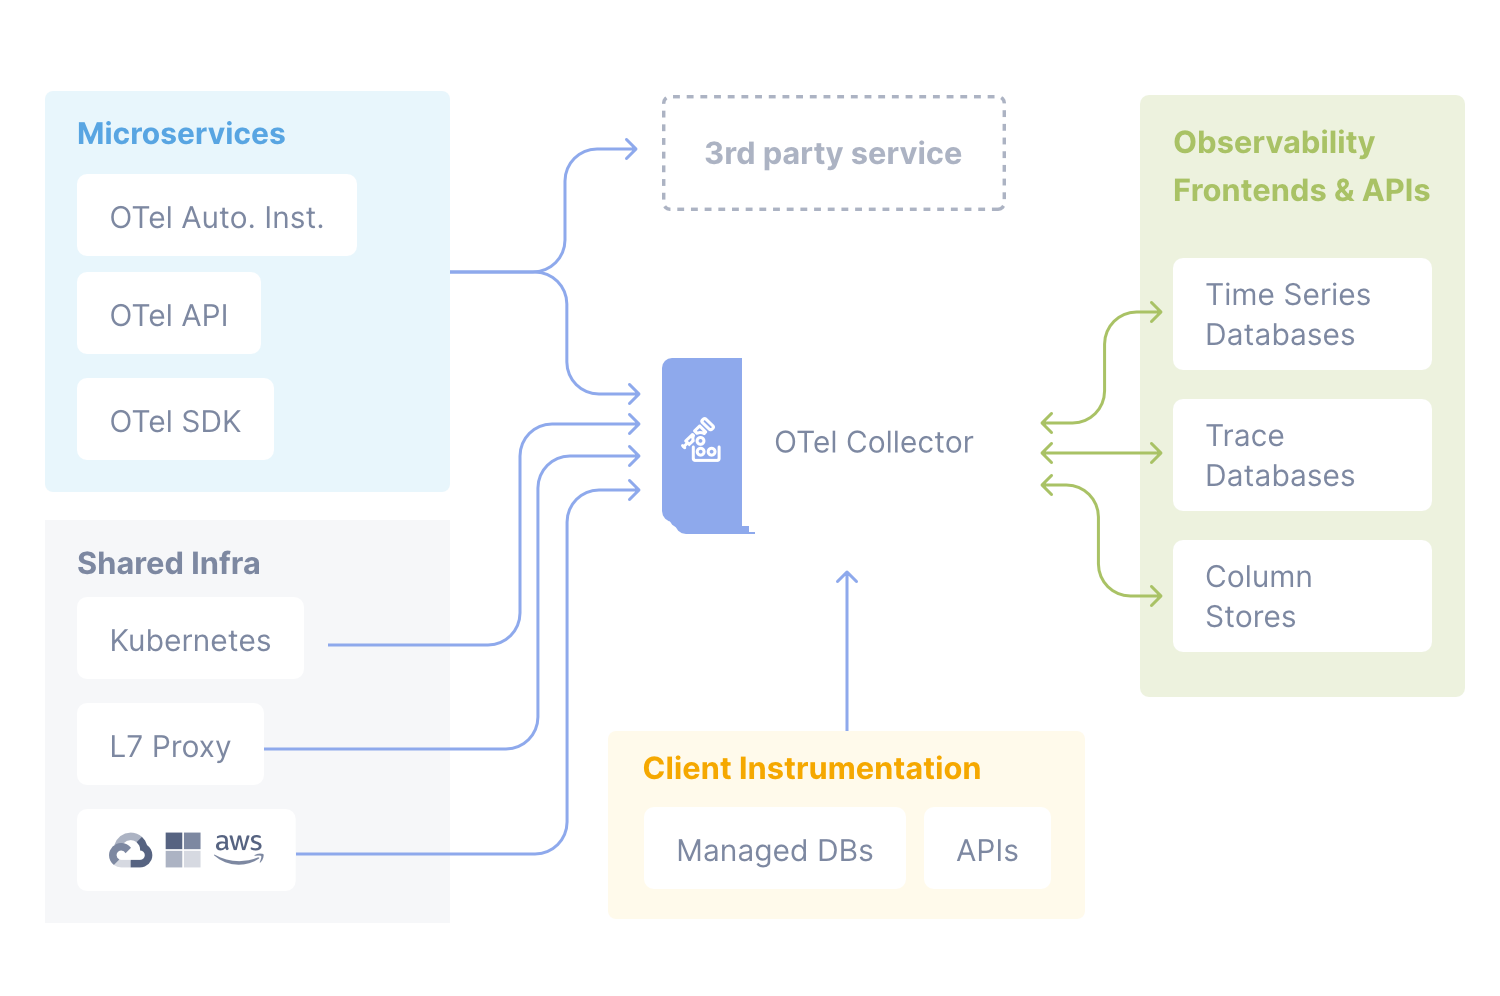
\includegraphics[width=12cm]{otel-diagram.png}
\centering
\caption{OpenTelemetry Reference Architecture.}
\label{fig:opentel-overview}
\end{figure}

Whilst tracing using a framework such as OpenTelemetry would be helpful in a larger production environment (Figure \ref{fig:opentel-overview} shows the architecture of OpenTelemetry\footnotemark{}), Omni currently only has four microservices.
Tracing has been ignored for the initial product but could easily be retrofitted around the existing logging infrastructure.
An OpenTel Exporter would then consume these traces from many different applications and publish them to a single location, for example, \underline{\href{https://prometheus.io}{Prometheus}} \nocite{prometheus}. 
The Kubernetes cluster provides top-level metrics covering basic needs, while load balancers provide more in-depth metrics, such as requests per second.
\footnotetext{`OpenTelemetry Reference Architecture' by OpenTelemetry Authors, from \url{https://opentelemetry.io/docs/}, licensed under \href{https://creativecommons.org/licenses/by/4.0/}{CC BY 4.0}.}

\section{Database}
\label{sec:impl-database}
Data is at the centre of every social media platform. The first step in creating Omni should be to build the database in which its data will be stored.
To ensure the database is reproducible on multiple servers (for example, when creating a new database shard), database migrations must be written and applied iteratively on top of one another until the final database structure has been formed. 
There are many tools and libraries for applying database migrations to a database, but since the microservices will be written in GoLang, the GoMigrate tool is a natural fit.

\subsection{Database Tables}
Figure \ref{fig:db-erd} shows the final design of the tables. The Omni platform has two main entities that are easy to see, and a third arises during the implementation.

\begin{figure}[htbp]
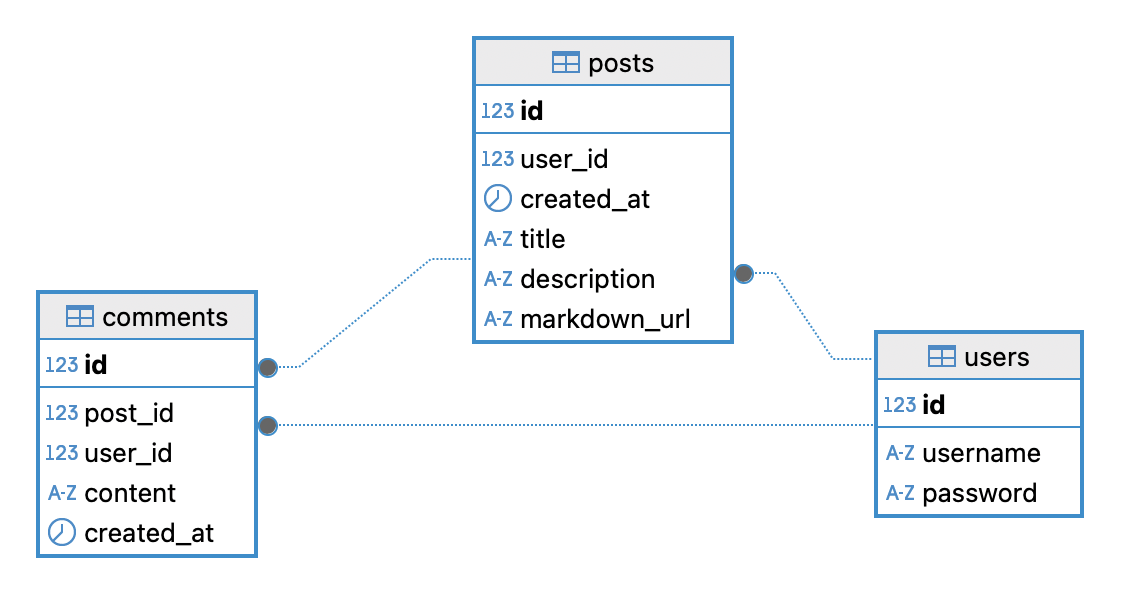
\includegraphics[width=12cm]{db-erd.png}
\centering
\caption{Database Entity Relationship Diagram}
\label{fig:db-erd}
\end{figure}

Information about each user needs to be stored, so a user table is naturally required. This includes any information about the user, such as username and password hash.
In the MVP of Omni, there is not much additional information stored about each user, but we could feasibly expand to store much more data for new features, such as storing a user's birthday.
In the future, if a hybrid approach for database distribution is used, a separate table to hold authentication data may be better to store this on a replicated database cluster rather than a sharded one.

The second easy-to-see table holds information about each post. It must store the creator's ID, title, description, link to the markdown file, timestamp, and more.
Posts will have a one-to-many relationship with users, where one user may create many posts, but each post is always associated with just one user. 

The final table is not as obvious to spot but still crucial: a table to store comments in. Storing this in the posts table does not make sense in a structured SQL database.
Adopting this approach could work in a NoSQL setup, but for popular posts, the document size would grow too big and slow down reading the post for everybody.
By storing the comments in a separate table, we can use pagination in our SQL queries to limit the number of comments we return to a user simultaneously.
This limits the load on the microservices, ensuring they are not overwhelmed by a very popular post with many comments.

\subsection{Discussion on Sharding}
As discussed in Section \ref{sec:design-system-database}, the design of the database and Snowflake IDs enable easy sharding of the database, whilst maintaining fast access times by backend microservices.
A single database has been used to maintain simplicity for the initial implementation and testing of the platform. The only difference this has in the code is that the logic for selecting which database node to retrieve data from is removed (as only one node contains all data).


\section{Backend Microservices}
\label{sec:impl-backend}
This section discusses how the backend microservices were created and how they interact with the broader environment.
Some patterns have been shared across services to enable as much code reuse as possible.

\subsection{Database Access}
\label{sec:impl-backend-db}
All three backend services require some level of database access. OmniAuth and OmniRead require only read access, whereas OmniWrite will read and write data. 

All the applications (currently) interact with the same database, although, as mentioned in Section \ref{sec:design-system-database-implementation}, future improvements could include using separate databases for things like authentication.
Because the database is shared, we can utilise the same database layer in each application, reducing the amount of code we need to write.

\subsubsection{The SQLc Library}
\underline{\href{https://sqlc.dev}{SQLc}} \nocite{sqlc} has been used to generate the database layer automatically.
This code generation library takes as input database migrations and all the queries to be run against the database.
It then compiles these inputs into type-safe code. There are multiple benefits to this approach:
\begin{itemize}
    \item Most of the code generated is boilerplate developers must write by hand or copy from documentation. It does not solve novel problems.
    \item The code generated is type-safe and handles embedding objects from joins for a more traditional object-orientated programming style. 
    \item The compiler flags breaking changes to the database via migrations when the database layer has been regenerated, but the business logic has not yet been modified.
\end{itemize}
Using this approach, SQLc has generated objects for users, posts, and comments, as well as other objects used when retrieving smaller data sections from each table.
Helpfully, the library generates an interface used within the code to access the database and an implementation of the interface for accessing the database.
However, this interface enables developers to write custom implementations, for example, to be used during unit testing. 

\lstinputlisting[language=Go, caption=The Generated GoLang Post Struct]{code-snippets/sqlc-go-models.go}

All the backend services share this database layer as there is no need to write the queries separately for each one, as operations like retrieving a user profile happen in all the services.

\subsubsection{Managing Database URLs}
In order for the services to make calls to the database, they need to know where to send requests.
This is defined by a URL that is passed to each application through the environment, allowing for on-the-fly changes to the configuration without having to rebuild each application. 
The start-up function parses this URL and then creates a database connection using Go's built-in \underline{\href{https://pkg.go.dev/database/sql}{database/SQL}} \nocite{gosqlpkg} package.
Finally, a Querier object (generated by SQLc) is initialised from the database connection object. This is the object which will be passed to each service's business logic so that database requests can be made.

\subsection{Authentication}
Authentication is an important part of any platform. It ensures that users can only access data and perform tasks they are authorised to do. 
Rather than using an authentication library, Omni uses a simple, custom authentication implementation, where users log in using a username and password.

\subsubsection{Sign Up}
\label{sec:impl-auth-signup}
When a user signs up to Omni, they enter a unique username and a password of their choice.
This information is sent to the backend, where the password is hashed using the bcrypt algorithm developed by \citeauthor{provos1999future}.
The GoLang package \underline{\href{https://pkg.go.dev/golang.org/x/crypto/bcrypt}{crypto/bcrypt}} \nocite{gobcryptpkg} handles this. The password hash is then stored in the database along with the rest of the user's details.

\subsubsection{Bcrypt}
The Bcrypt algorithm stores all the information required to verify a password attempt in the hash.

\begin{figure}[htbp]
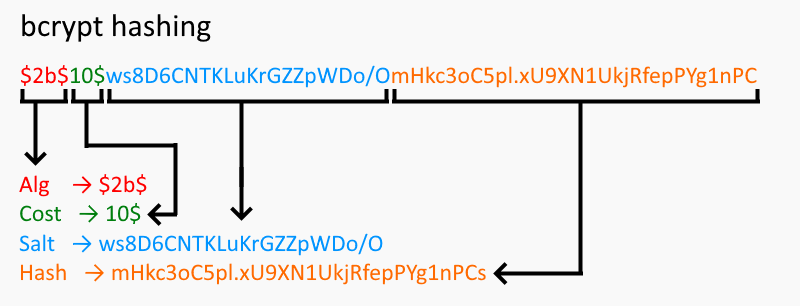
\includegraphics[width=12cm]{bcrypt-parts.png}
\centering
\caption{Sections of the Bcrypt Hash}
\end{figure}

The first section of the hash contains the algorithm used to create it. Bcrypt uses a version of the Blowfish cypher, denoted by the hash \verb|$2b$|.
The second section is the cost factor used in the algorithm. The default of 10 is used for Omni, but in production, this should be increased to 12 or higher.
Generally, the larger the value of the cost factor, the slower it is to check a password.
While counter-intuitive, this is the desired behaviour, as the slower it is to check a password, the harder it is for a brute-force algorithm to check the most common passwords.
The third section of the hash is the salt used; this is stored as plain text so that it can be used to derive the encryption key for later use.
Finally, the encrypted password is stored as the last part of the hash, which is compared against a potential password.

Checking a password involves deriving the encryption key from the given algorithm, cost factor and salt, using that key to encrypt the given password and then comparing it against the valid password hash. If the hashes match, the password is valid.

\subsubsection{JSON Web Tokens}
JWTs are the industry standard for ongoing authentication. They can contain many standard or custom `claims', which the application uses to determine whether the JWT is valid.
In particular, Omni uses the \verb|exp| and \verb|sub| claims (standing for expires at and subject, respectively). 

After a JWT body is generated, applications hash it using a secret key, which is appended to the JWT to ensure that the body is not modified by anyone other than the authorised applications. 
Figure \ref{fig:jwt-parts} shows the three sections of a JWT.

\begin{figure}[htbp]
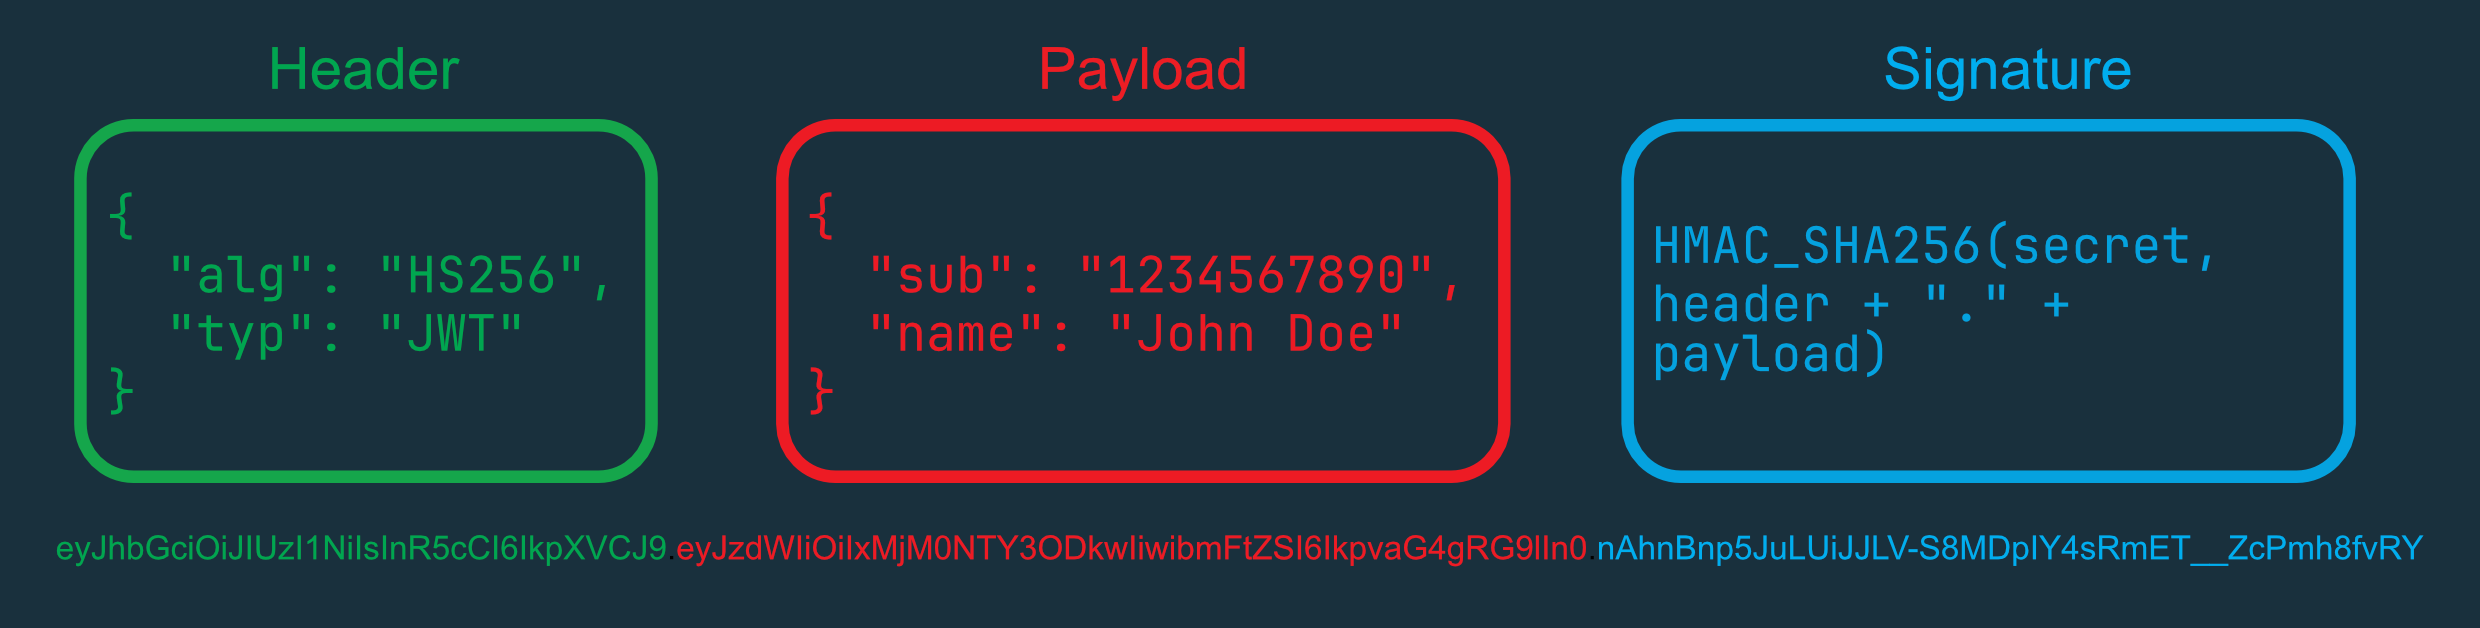
\includegraphics[width=12cm]{jwt-parts.png}
\centering
\caption{Sections of a JSON Web Token}
\label{fig:jwt-parts}
\end{figure}

In subsequent requests to restricted endpoints, clients attach their JWT in the Authorization header of the HTTP request.
The relevant backend, which handles requests to that particular endpoint, can then verify the claims in the JWT.
Based on the subject claim of the JWT, the backend can decide if the client making the request is authorised to do so for the particular action they are performing.
For example, a user can delete a post they have created but cannot delete posts from other users.

\subsection{OmniAuth}
The simplest of the backend services is OmniAuth, which authenticates an existing user to access restricted endpoints.
OmniAuth serves just one endpoint: \verb|POST /api/login|. The handler expects the request to have a JSON body with the fields \verb|username| and \verb|password|. 
The username is used to retrieve the user from the database. When the user does not exist, the endpoint returns a 404 Not Found HTTP error.
The returned data from the database includes the Bcrypt hash of the user's password. 

As mentioned above in Section \ref{sec:impl-auth-signup}, the \underline{\href{https://pkg.go.dev/golang.org/x/crypto/bcrypt}{crypto/bcrypt}} \nocite{gobcryptpkg} package compares the password sent in the request to the hashed password stored in the database.
If the passwords match, the authentication request is valid. If they do not match, the request returns a 401 Unauthorised HTTP error.

Given that the passwords match, OmniAuth will create a JSON Web Token (JWT) (code shown in Listing \ref{lst:go-jwt}) that can be used to authenticate the user for subsequent requests to restricted endpoints.

\lstinputlisting[language=Go, caption=Example of Creating a JWT, label={lst:go-jwt}]{code-snippets/go-jwt-creation.go}

\subsection{OmniRead}
OmniRead, as described in Section \ref{sec:design-system-backend}, is responsible for handling any HTTP Get requests. This allows us to scale read requests separately from the scaling of backend services that handle write requests.
In the initial version of Omni, the data that users need to be able to read is: 
\begin{itemize}
    \item Posts
    \item Users
    \item Comments
\end{itemize}
However, we have more than three endpoints, as users may want to access different data sections differently. For example, a user may want to retrieve all the posts a user has created and the most recent posts by any user. 

All the API endpoints served by OmniRead are unauthorised, meaning that anybody can access them without a JWT token. This simplifies the service regarding the middleware required for each endpoint and its runtime configuration in the Kubernetes environment. 

For some endpoints that could return infinite amounts of data, such as retrieving comments on a post or posts by a particular user, paging is needed.
This ensures that the database and the backend service are not overwhelmed by a denial-of-service attack, where a malicious request can cause the entire service to hang or run out of memory while processing it. 
Paging ensures that the data returned has a maximum size of ten items. Users who wish to see more items can request the next page, which will return the following ten items.

Achieving this paging in the application layer is trivial, but it still leaves the attack vector open. In this scenario, the application layer would still require all the data from the database, even if it only returned a subset to the user. 
Luckily, popular SQL databases already have this paging feature built-in through the \verb|LIMIT| and \verb|OFFSET| keywords.
\verb|LIMIT|, as the name suggests, limits the number of rows of data returned, and \verb|OFFSET| skips the number of rows specified.
For example, with a \verb|LIMIT| of 10 and \verb|OFFSET| of 0, the first 10 rows will be returned. With an \verb|OFFSET| of 10, rows 11-20 are returned. 

\lstinputlisting[language=SQL, caption=Example of SQLc Query with LIMIT and OFFSET]{code-snippets/sql-limit-example.sql}

Other paging strategies also exist. For example, in the context of comments, a user may prefer to page by time, finding all the comments before or after a timestamp.
This paging application is more useful for other applications that use the API, perhaps for research purposes.
In contrast, users interacting with the Omni platform via the website will likely want to read the most recent comments on a post or the highest-rated comments if a liking system is introduced.
The \verb|LIMIT| and \verb|OFFSET| approach is more efficient for these cases when compared to the client specifying a timestamp or other parameter to find comments before or after, with different sorts applied to the query. 

OmniRead returns data in the response body in a JSON format. JSON is the standard format for transmitting data in APIs on the web.
Whilst other more efficient formats exist, such as \underline{\href{https://protobuf.dev}{ProtoBuf}} \nocite{protobuf}, JSON is ubiquitous and well-supported by most languages' standard libraries.
GoLang has powerful, built-in tooling to encode and decode to and from the JSON format into standard GoLang structs.
As part of a set of helper functions for all the backend services, Omni has a helper function that takes an object and an HTTP Response Writer object and writes the JSON encoding of the object to the response along with a 200 Success HTTP code.
This helper function is used across all the backend services to transmit data to the request sender. 

\lstinputlisting[language=Go, caption=Example of Writing JSON to the Response, label={lst:go-json}]{code-snippets/encode-json-helper.go}

\subsubsection{Conforming to the HTTP Specification}
Throughout the OmniRead service (and all the backend services), Omni attempts to conform as much as possible to the uniform HTTP interface defined by \citeauthor{fielding1999rfc2616}.
In practice, this means reflecting as much information as possible through HTTP Status Codes and adopting the correct HTTP verbs.
Some examples include 200 Success and 201 No Content when requests are successful, with the former indicating there is some returned content in the body of the response, whilst the latter means nothing was returned.
When a request is malformed or otherwise incorrect, status codes in the range 4XX are returned depending on the type of error.
Finally, the service returns 500 Internal Server Error and 503 Service Unavailable errors when the backend encounters errors it cannot recover from, such as the database being down. 

Consumers of the API should be able to use HTTP Status Codes as the first port of call to immediately know if a request was successful, rather than the way that some more modern JavaScript frameworks hide errors inside of 200 Success messages.
The practice of hiding errors inside responses that return with a 200 code can lead to poor error handling and unexpected fatal crashes.

As discussed by \citeauthor{richardson2008restful}, ``when the method information isn’t found in the HTTP method, the interface stops being uniform.''
It is important to conform as much as possible to the specifications that underpin the modern web; otherwise, the tooling and developers working on the web will have to work harder to achieve the same baseline of safety.
